\chapter{One-time pad}

Un cifrario è perfetto se, una volta scelto il cifrario (o progettato), occorre valutare la sua sicurezza (quanto è resistente agli attacchi). Abbiamo due metodi classici che ci permettono di capire se un cifrario è robusto. Ovvero
\begin{itemize}
	\item Protocollo a chiave segreta (metodo empirico) : si distribuisce agli scienziati il cifrario, se dopo tot tempo nessuno lo viola significa che è sicuro. Probabilmente è sicuro però, sarebbe più opportuna una dimostrazione pratica che dimostra che il protocollo non è violabile (staremmo più tranquilli).
	\item (metodo formale) : Dimostro che, quel protocollo crittografico non è sicuro, però per violarlo è necessario disporre di una determinata quantità di risorse (tempo di calcolo). Se le risorse sono inarrivabili, il protocollo è sicuro ed è migliore del metodo empirico esposto nel punto precedente.
\end{itemize}

Il one-time-pad è un esempio di cifrario perfetto, in cui riusciremo a dimostrare (cosa rara nei cifrari), che in determinate situazioni, il cifrario non è violabile, con qualsiasi quantità di risorse a disposizione. Problema : è troppo costoso, è quasi inutilizzabile, tranne in certi casi specifici (molto ristretto).
Introduce però alcuni concetti che saranno utili nel proseguo del corso.

\section{Esistono cifrari inviolabili?}

Inviolabile = qualcuno intercettando il crittogramma che passa sul canale di comunicazione, riesce a risalire al messaggio? Anche conoscendo le funzioni di cifratura/decifratura? Considerando che l'unica cosa che non conosciamo è la chiave segreta.
\\
La risposta è : esistono cifrari inviolabili, come ad esempio il one-time-pad ma l'impiego è quasi impossibile per via del loro altissimo costo. Dunque fra i cifrari che si utilizzano in pratica non esistono quelli inviolabili, si utilizzano invece cifrari sicuri ed economici e che vengono utilizzati ogni giorno per comunicazione di massa(acquistiamo efficienza e perdiamo sicurezza).

\section{Processo stocastico (Modello matematico)}
Abbiamo una comunicazione tra mittente (Mitt) e destinatario (Dest), questa comunicazione è modellata come un processo stocastico (ovvero probabilistico), in cui il comportamento del mittente è descritto da una variabile aleatoria M (assume certi valori con una determinata probabilità). Valori assunti da M = possibili messaggi. I possibili messaggi vengono presi dallo spazio dei messaggi (msg). Abbiamo un canale, dove viaggia il crittogramma corrispondente al messaggio dopo averlo codificato e sul canale abbiamo una variabile aleatoria C, che assume i valori dei crittogrammi generati a partire dai messaggi. 
In sintesi : 
\begin{itemize}
	\item M : variabile aleatoria;
	\item m : valore assunto dalla variabile aleatoria in un tempo t;
	\item C : processo che trasforma il messaggio; 
	\item c : crittogramma generato a partire dal messaggio, C(m) = c. il crittogramma è un valore possibile del canale. Quando m viene codificato con C, sul canale leggo c.
\end{itemize}
La distribuzione di probabilità della M dipende dalla sorgente, chi è la sorgente? la sorgente è colui che genera il messaggio (tira fuori i bit, che vengono organizzati in blocchi e poi spenditi sul canale).

\paragraph{Nota :} Non è possibile che due messaggi uguali generino due c diverse, allo stesso modo non è possibile che due messaggi diversi abbiano uno stesso c, dal momento che in quel caso il destinatario non sarebbe in grado di ottenere con precisione il messaggio in seguito alla codifica.\\\\
Esempio applicativo : 
Il mittente è il signor dado, che vuole spedire un messaggio al destinatario. I messaggi che spedisce il signor dado sono $M = \{1, 2, 3, 4, 5, 6\}$. Il modello matematico dice che io spedisco $1 con p = 0.5; (2, 4, 5, 6) con p = 0.1$ (questa è la distribuzione di probabilità del nostro mittente dado). Quando dado vuole spedire $4$, prende la sua codifica e la cifra, $C(4)$, che genererà un crittogramma $c$ che poi verrà spedito sul canale. Chi guarda il canale (ad esempio l'intruso), prima che passi $c$, sa già che il messaggio 4 esce con probabilità 0.1, stessa cosa per ogni valore. Ora supponiamo di aver letto $c$, noi vogliamo che conoscendo $c$ la probabilità che il messaggio fosse 4 rimanga sempre 0.1, questo vuol dire che l'informazione rivelata dall'evento "ho letto $c$" è nulla, non serve a nulla. Un cifrario è perfetto se la probabilità iniziale rimane inalterata anche se viene visto ciò che è passato sul canale di comunicazione.

\subsection{Notazione}

$P(M = m)$ = $\{$ con quale probabilità il mittente vuole spedire il messaggio $m$ $\}$ .  \\
$P(M = m | C = c)$ = $\{$ con che probabilità il mittente ha spedito il messaggio $m$, sapendo che sul canale abbiamo letto il crittogramma $c$. $\}$

\paragraph{Deduciamo che} Se le due probabilità sono uguali, abbiamo che la lettura del crittogramma $c$ non mi ha dato nessuna informazione riguardo il messaggio che è stato spedito (concetto di indipendenza : $P(A|B) = P(A)$).

\section{Scenario ipotetico}

Il crittoanalista conosce la distribuzione di probabilità con cui il mittente genera il messaggio, il cifrario e lo spazio k delle chiavi, l'unica cosa che non conosce è la chiave che è stata utilizzata (la chiave segreta). \\
Secondo Shannon il cifrario è perfetto quando, per ogni $m \in Msg$ e $c \in Crittogrammi$, vale la relazione :  $P(M = m | C = c) = P(M = m)$.
Supponendo di avere messaggi composti dalla coppia nome+cognome, non mi basta che l'intruso non sappia nè nome nè cognome, non voglio nemmeno che l'intruso scopra se l'utente sia maschio o femmina, non voglio che vengano capite nemmeno caratteristiche legate al messaggio.
\subsection{Descrizione scenario}
Supponiamo di avere dei messaggi contenenti la coppia <nome, cognome> e che tutte le coppie siano equiprobabili. Supponiamo inoltre che sulla terra ci siano 1000 coppie <nome, cognome>. Supponiamo inoltre che sul pianeta terra ci siano 300 maschi e 700 femmine. Senza leggere nulla sul canale quale è la probabilità che sia spedito un certo <nome, cognome>? 1/1000. Se io invece leggo il crittogramma c e riesco a capire che si tratti di una femmina, la probabilità varia! Perchè la probabilità che il nome contenuto nel messaggio sia <Luigi, Rossi> diventa pari a 0, perchè Luigi è un nome maschile. In un contesto perfetto, questo non deve accadere.

\section{Numero di chiavi in un cifrario perfetto}
La prima dimostrazione formale la si può fare sulla base che:
In un cifrario perfetto, il numero delle chiavi possibili deve essere maggiore o uguale al numero dei messaggi possibili. \\\\
Vuol dire che se io voglio spedire messaggi lunghi 100 bit, noi sappiamo che i messaggi lunghi 100 bit sono $2^{100}$. Ora dimostriamo che, se il cifrario è perfetto, allora io ho bisogno di almeno $2^{100}$ chiavi. In sostanza le chiavi devono cifrare i messaggi, nascondendo tutte le possibili informazioni, di conseguenza ne servono tante.
\subsection{Dimostrazione formale}
Sia $N_m$ il numero di messaggi possibili, cioè tali che $P(M = m) > 0$ e sia $N_k$ il numero di chiavi possibili. Poniamo per assurdo che $N_m > N_k$, se questo è vero, esiste un crittogramma $c$ con $P(C = c) > 0 $ (ovvero con probabilità che passi sul canale) a cui corrispondono $s \leq N_k$ messaggi (non necessariamente distinti), ottenuti decrittando $c$ con tutte le possibili chiavi. Poichè $N_m \geq N_k \geq s$, esiste almeno un messaggio $m$ con $P(M = m | C = c) = 0 \neq P(M = m)$, ovvero per $N_m > N_k$ il cifrario \textbf{non} è perfetto.

\begin{figure}[htp]
	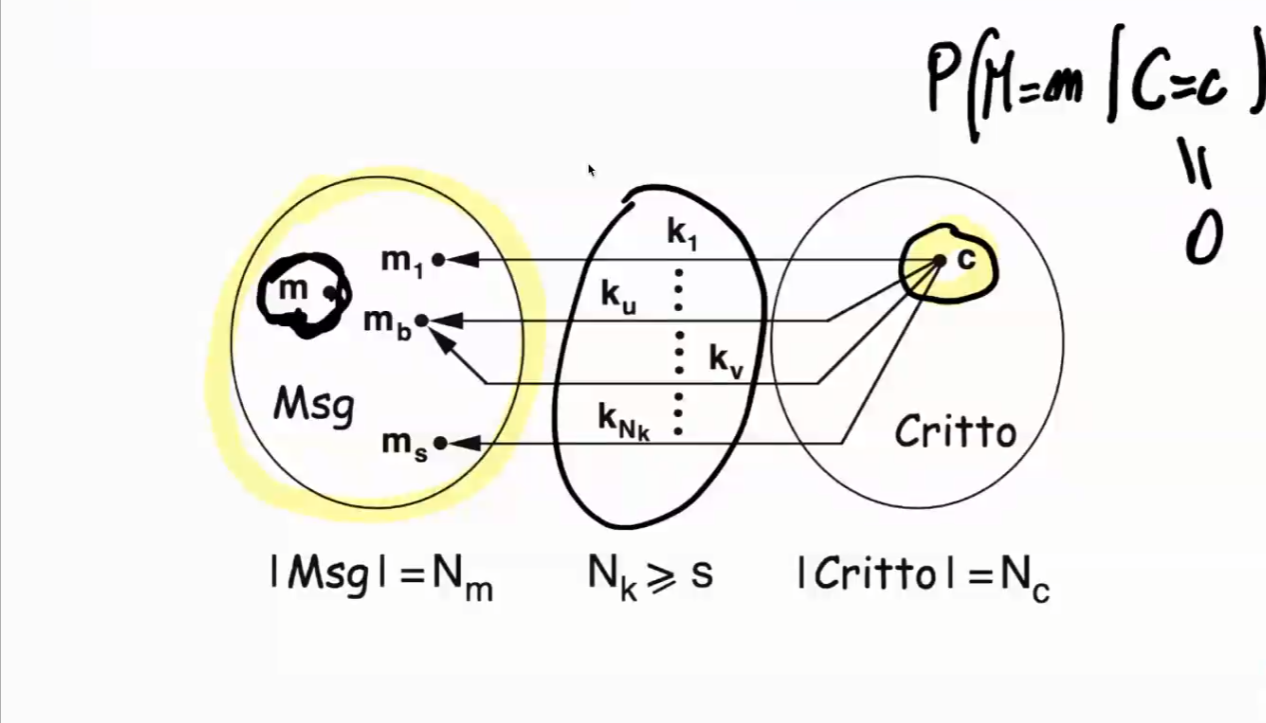
\includegraphics[width=0.8\linewidth]{./img/teorema1.png}
	\caption{Nell'immagine viene esplicitato il ragionamento, si nota che m rimane da solo, in assenza di chiavi con cui crittografare il messaggio. Questo comporta che la $P(M = m)$ non è indipendente rispetto $P(M = m | C = c)$, dunque non si tratta di un cifrario perfetto.}
	\label{img:teorema1}
\end{figure}

\section{Deduzione logica}
Conseguentemente alla dimostrazione, otteniamo che, in un cifrario perfetto, il numero delle chiavi deve essere maggiore o uguale al numero dei messaggi possibili. Questo ci dice che i cifrari perfetti sono inutilizzabili, perchè in questo caso, se devo spedire 1 gb di messaggio, ho necessità di 1 gb di chiave ed è molto oneroso. Ci dice inoltre che se le chiavi si consumano, un messaggio di 56 bit, una volta spedito, consuma i 56 bit di chiave, dunque non può essere riutilizzata. Dal momento che le chiavi più sicure sono quelle random, inizia a maneggiare in noi il fatto che la randomness sia una risorsa, dunque avere bit a disposizione rappresenta una risorsa (e se usiamo, come in questo caso, chiavi usa e getta, la perdiamo, il cifrario diventa poco robusto). .

\section{One-Time Pad}
L'one-time-pad veniva usato durante la guerra fredda (Washington e Mosca), perchè la comunicazione non era così frequente (e le chiavi non si consumavano così in fretta), più si riciclano le chiavi, più il protocollo è imperfetto.
\subsection{Funzionamento}
Si costruisce una chiave segreta:
Si costruisce una sequenza di bit $k = k_1, k_2, ..., k_n$, nota al mittente e al destinatario. Supponiamo di voler inviare un messaggio più corto di questa chiave e che la chiave sia scelta a caso ((p bit a 0)/(p bit a 1) = 0.5).\\\\
Cifratura:
Il messaggio da trasmettere $m = m_1, m_2, ..., m_n$, il crittogramma $c = c_1, c_2, ..., c_n$ lo si ottiene eseguendo uno xor fra $m$ e $k$, per ogni $i$. \\Decifratura : Riapplicando lo xor al $c$ risultante riottengo il messaggio originale.

\begin{figure}[htp]
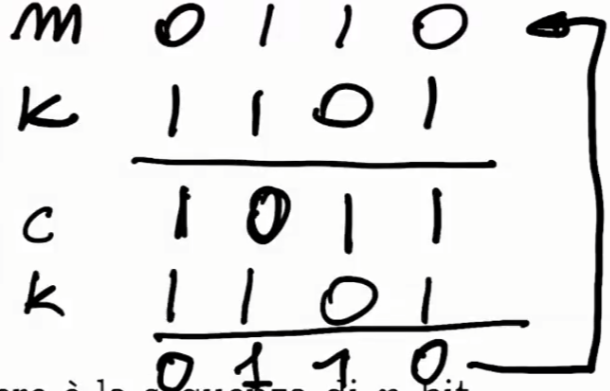
\includegraphics[width=0.8\linewidth]{./img/xor.png}
\label{img:xor}
\end{figure}
Dove sta il trucco?? Sta nel fatto che i bit di $k$, essendo generati a caso, cancellano l'informazione contenuta nel messaggio (dunque un intruso cosa può dire del messaggio? nulla, la chiave lo ha obliterato).

\subsection{Dimostrazione perfezione One time pad}
Per semplicità assumiamo che:
\begin{itemize}
	\item tutti i messaggi abbiano la stessa lunghezza n;
	\item tutte le sequenze di n bit sono messaggi possibili (messaggi possibili = tutte le possibili permutazioni della sequenza di bit).
\end{itemize}
\subsubsection{Enunciato}
Utilizzando una chiave scelta totalmente a caso per ogni messaggio, il cifrario One-Time pad è perfetto ed impiega un numero minimo di chiavi.
\subsubsection{Dimostrazione}
Per dimostrare l'enunciato è sufficiente dimostrare che $P(M = m | C = c) = P(M = m)$. E' possibile farlo applicando il teorema di bayes, per il quale :\\\\
$P(M = m | C = c) = \dfrac{P(M = m, C = c)}{P(C = c)} = \dfrac{P(C=c | M = m) P(M = m)}{P(C = c)}$\\\\
Osserviamo ora che l’evento $\{M = m; C = c\}$ descrive la situazione in cui Mitt ha generato il messaggio $m$ e l’ha cifrato come crittogramma $c$. Per la definizione di XOR, fissato il messaggio, chiavi diverse danno origine a crittogrammi diversi, e ogni chiave può essere generata, in maniera randomica, con probabilità $(\dfrac{1}{2})^n$ (questo perchè o il bit è 0 o 1, per una sequenza di $n$ elementi ed è random). Dunque, fissato $m$, risulta $P(C = c)$ = $(\dfrac{1}{2})^n$ per ogni $c$, ovvero una costante, questo comporta che i due eventi siano indipendenti. Di conseguenza si giunge alla conclusione che (seguendo tutti i passaggi):\\

$P(M = m | C = c) = \dfrac{P(C=c | M = m) P(M = m)}{P(C = c)} = \dfrac{P(C = c) P(M = m)}{P(C = c)} = P(M = m)$.

\paragraph{Inoltre} è implicitamente dimostrato che Il numero di chiavi non può essere inferiore al numero di messaggi. Nel One-Time Pad il numero di chiavi è 2n
che è uguale al numero di messaggi (non ne possiamo avere di meno).
